\documentclass{beamer}
\mode<presentation>{
\usetheme{Amsterdam}
\setbeamertemplate{navigation symbols}{}}
\usepackage[utf8]{inputenc}
\usepackage{graphicx}
\usepackage{booktabs}
\usepackage{circuitikz}
\usepackage{tikz}
\usetikzlibrary{matrix,calc}
\usetikzlibrary{positioning}

%----------------------------------------------------------------------------------------
%	TITULOS
%----------------------------------------------------------------------------------------
\title[Seminario de tecnologia]{Unidad V\\ Big Data y Analytics}
\author{David A. Trejo Pizzo}
\institute[Instituto Multimedial Da Vinci]
{Departamento de sistemas\\
\medskip
\textit{dtrejopizzo@gmail.com}}
\date{Marzo, 2015}
\begin{document}
\begin{frame}
\titlepage
\end{frame}


%----------------------------------------------------------------------------------------
%	INDICE
%----------------------------------------------------------------------------------------
\begin{frame}
\frametitle{Estructura}
\tableofcontents
\end{frame}


%----------------------------------------------------------------------------------------
%	SLIDES
%----------------------------------------------------------------------------------------

\section{Introducción}

\begin{frame}
\frametitle{Adquisición de datos}
\begin{itemize}
\item 
\item 
\item 
\end{itemize}
%\begin{figure}[!h]
%\centering
%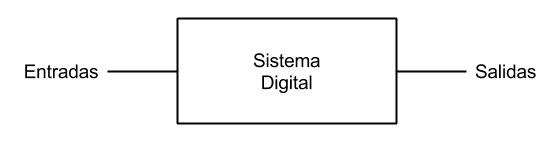
\includegraphics[width=2in]{sistemad}
%\end{figure}
\end{frame}
%------------------------------------------------

\begin{frame}
\frametitle{Sensores}
\begin{itemize}
\item Es un dispositivo capaz de detectar magnitudes físicas o químicas, llamadas variables de instrumentación (impulsos), y transformarlas en variables eléctricas.
\end{itemize}
\end{frame}
%------------------------------------------------

\begin{frame}
\frametitle{Tensiones digitales}
\begin{itemize}
\item 
\item 
\end{itemize}
\end{frame}
%------------------------------------------------

\section{Álgebra de Boole}
\begin{frame}
\frametitle{}

\end{frame}
%------------------------------------------------

\begin{frame}
\frametitle{}

\end{frame}
%------------------------------------------------

\section{Compuertas}

\begin{frame}
\frametitle{}

\end{frame}
%------------------------------------------------

\begin{frame}
\frametitle{}

\end{frame}
%------------------------------------------------

\begin{frame}
\frametitle{}

\end{frame}
%------------------------------------------------

\begin{frame}
\frametitle{}

\end{frame}
%------------------------------------------------

\begin{frame}
\frametitle{}

\end{frame}
%------------------------------------------------

\begin{frame}
\frametitle{}

\end{frame}
%------------------------------------------------

\begin{frame}
\frametitle{}

\end{frame}
%------------------------------------------------


\section{Logica combinacional}

\begin{frame}
\frametitle{}

\end{frame}
%------------------------------------------------

\begin{frame}
\frametitle{}

\end{frame}
%------------------------------------------------

\section{Logica secuencial}

\begin{frame}
\frametitle{}

\end{frame}
%------------------------------------------------

\begin{frame}
\frametitle{}

\end{frame}
%------------------------------------------------

\begin{frame}
\frametitle{}

\end{frame}
%------------------------------------------------

\begin{frame}
\frametitle{}

\end{frame}
%------------------------------------------------

\begin{frame}
\frametitle{}

\end{frame}
%------------------------------------------------

\end{document}